\section{Real-world implementation and experiments}\label{sec:exp}
In this section, real-world implementation of the two approaches to perform the backflip maneuver with the Crazyflie 2.1 drone, the experimental setup, and measurement results are presented. The experimental setup consists of the quadcopter with on-board sensors and microcontroller units (MCUs), the OptiTrack motion capture system, OptiTrack server, and ground control PC. The block diagram of the setup is displayed in Figure~\ref{fig:sys} with the direction and content of the information flow between the components.

\begin{figure}[b]
\centering
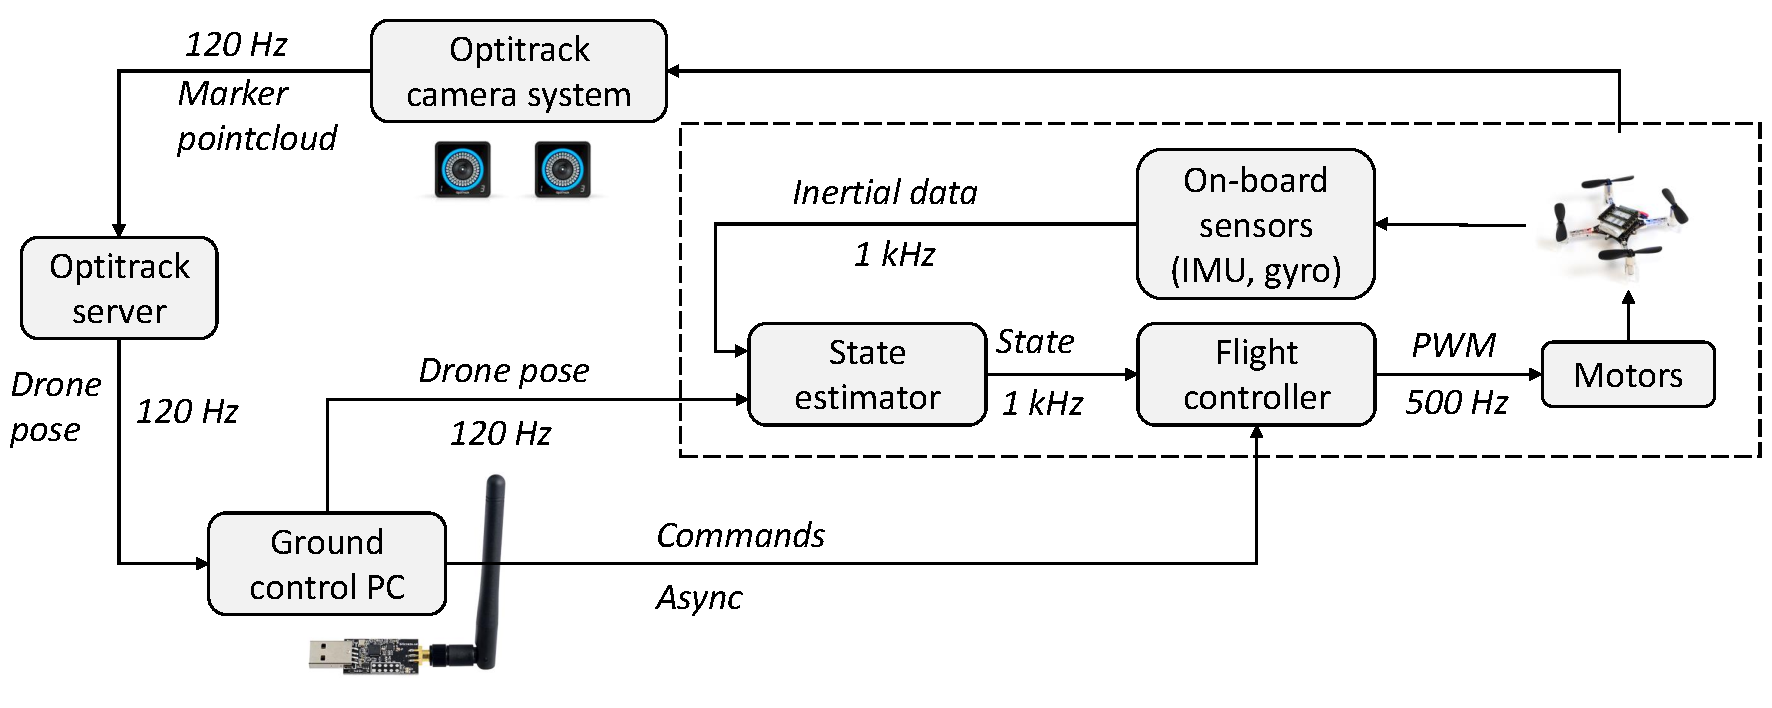
\includegraphics[width=.8\textwidth]{Fig/system.pdf}
\caption[Block diagram of the experimental setup]{Block diagram of the experimental setup: indoor quadcopter navigation with internal and external measurement system.}
\label{fig:sys}
\end{figure}

\subsection{The Bitcraze Crazyflie 2.1 drone}
This subsection presents an overview of the hardware and software of the Crazyflie 2.1 nano quadrotor, developed by the Swedish company Bitcraze AB. The vehicle is designed to be a development platform for research and education, therefore it is both fully open source and open hardware. Firstly the hardware specifications are summarized, and afterwards the structure of the firmware and control implementation possibilities are discussed.

\subsubsection{Hardware}

The quadcopter is an out-of-the-box device, the user only needs to assemble the parts. The central unit contains IMU sensors with accelerometer, gyroscope, magnetometer and barometer, and two microcontrollers: a STM32F405 for running the main application (e.g. state estimator, controller), and a nRF51822 for radio communication and power management. The four 4.2 V coreless BDC motors are connected to the central unit with plastic motor mounts. The propellers are fixed to the motor shafts using interference fit, and a 250 mAh LiPo battery is connected to the central unit to provide electric power. The drone weighs 28 grams, and the propeller-to-propeller distance is 92 millimeters.

Using the stock battery the flight time is 7 minutes without any external payloads. The maximum recommended payload is 15 grams including the extension decks which can be mounted to the drone. We only use one extension deck, on which the OptiTrack markers are mounted (see Fig. \ref{fig:hardware}), but there are several possibilities to extend the functionality and visual effects, for example the flow deck for optical flow measurement or the LED-ring deck.

The workstation PC communicates with the drone via the Crazyradio PA 2.4 GHz USB dongle. The radio communication makes it possible to update the firmware without a cable, and communicate with the quadrotor mid-flight, i.e. send external position data, update parameters, or log measurement data. The main parts of the hardware are displayed in Figure \ref{fig:hardware}.


\begin{figure}
\centering
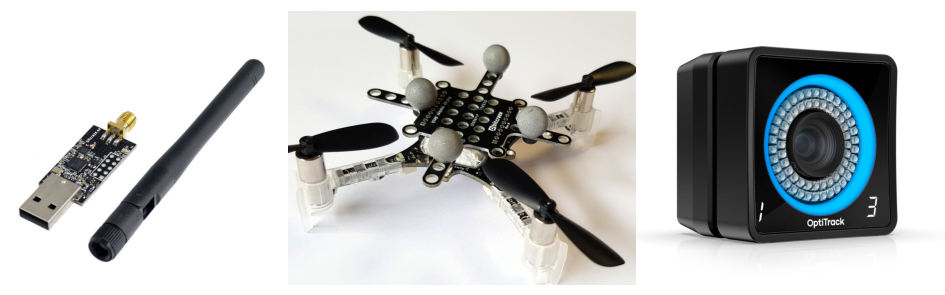
\includegraphics[scale=.6]{Fig/hardware.pdf}
\caption{The Crazyradio PA, Crazyflie 2.1 with motion capture markers, and an OptiTrack Prime 13 camera.}\label{fig:hardware}
\end{figure}

\subsubsection{Software}
The open-source software continuously developed by Bitcraze\footnote{\url{https://www.bitcraze.io/documentation/repository/}} includes the firmware, a Python client application and Python library with examples. In addition, we use the Crazyswarm platform \cite{crazyswarm} to easily handle the high-level control of multiple drones simultaneously, the OptiTrack measurement data, logging, and communication.

Out of all software components, we mostly use the firmware written in C language to implement our on-board controller, and the Python API for high-level commands and computation. The nRF51822 microcontroller manages the communication and power distribution, in which areas the default implementation is sufficient for us. However, the firmware of the STM32F405 contains the stabilizer unit responsible for handling high-level commands, state estimation and control input calculation. Two state estimators are implemented in the stock firmware of the Crazyflie: a complementary filter and extended Kalman filter. We use the latter, as it is more accurate for the fusion of internal and external sensor data.

There are three built-in controllers in the default firmware, a cascaded PID controller, the Mellinger controller \cite{mellinger2011}, and the  Incremental Nonlinear Dynamic Inversion (INDI) controller \cite{indi2015}. In this project, we use the PID controller for setpoint stabilization before and after the open-loop flip maneuver. Our own implementation of the geometric controller is responsible for backflipping with pitch reference, setpoint stabilization, and more complex, aggressive trajectory tracking.

%The structure of the cascaded PID controller is built as follows. The outermost loop is position control, which receives and handles the position or velocity input from the commander, running at 100 Hz. The next cascade is the attitude controller, which takes the error of the desired attitude as an input from the sensors, and outputs the desired attitude rate, running at 500 Hz. The innermost loop is the attitude rate controller, which also runs at 500 Hz. It receives the filtered output of the gyroscope rates, and outputs the collective thrust and the three torques in \eqref{eq:inputs} directly to the power distribution module.


% \begin{figure}
% \centering
% 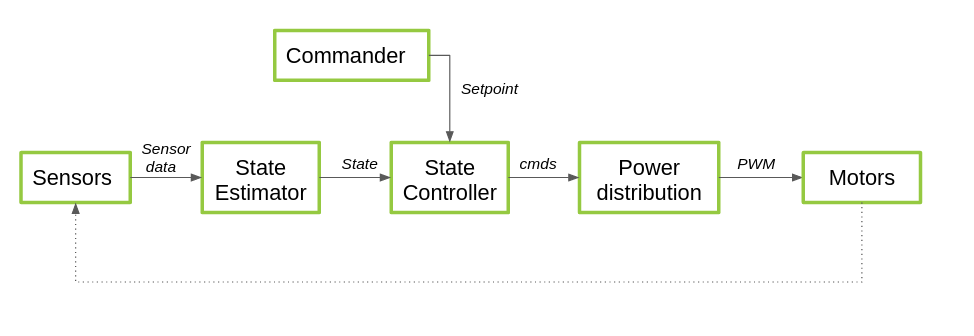
\includegraphics[width=\textwidth]{Fig/sensors_to_motors.png}
% \caption{Structure of the stabilizer module.}
% \label{fig:stab}
% \end{figure}



%\begin{table}[!h]
%\centering
%\begin{tabular}{l|c|c}
%mass & $m$ & 28 g\\
%\hline
%prop-to-prop length &$ l$ & 92 mm\\
%\hline

%\end{tabular}
%\caption{Physical parameters of the Crazyflie 2.1}
%\end{table}

\subsection{OptiTrack motion capture system}
At SZTAKI AIMotion Lab, we use OptiTrack for the real-time pose measurement of the drones which is a high precision motion capture system with submillimeter resolution. The system includes six Prime 13 infrared cameras sending the position information of specific markers at 120 Hz. Using the Motive software of OptiTrack, we can define rigid bodies with unique identifiers (both drones and obstacles), and broadcast their position and orientation information directly through local network.

Although OptiTrack is a very precise and efficient measurement device, sometimes it is not easy to arrange the markers on the drone such that at least four cameras see them at all times, especially during the flip maneuver. In these situations, the state estimator of the drone automatically switches to use only the information of the inertial measurement unit, which is sufficient for hovering and attitude stabilization.


\begin{figure}
\centering
\setlength{\fboxsep}{0pt}%
\setlength{\fboxrule}{1pt}%
\fbox{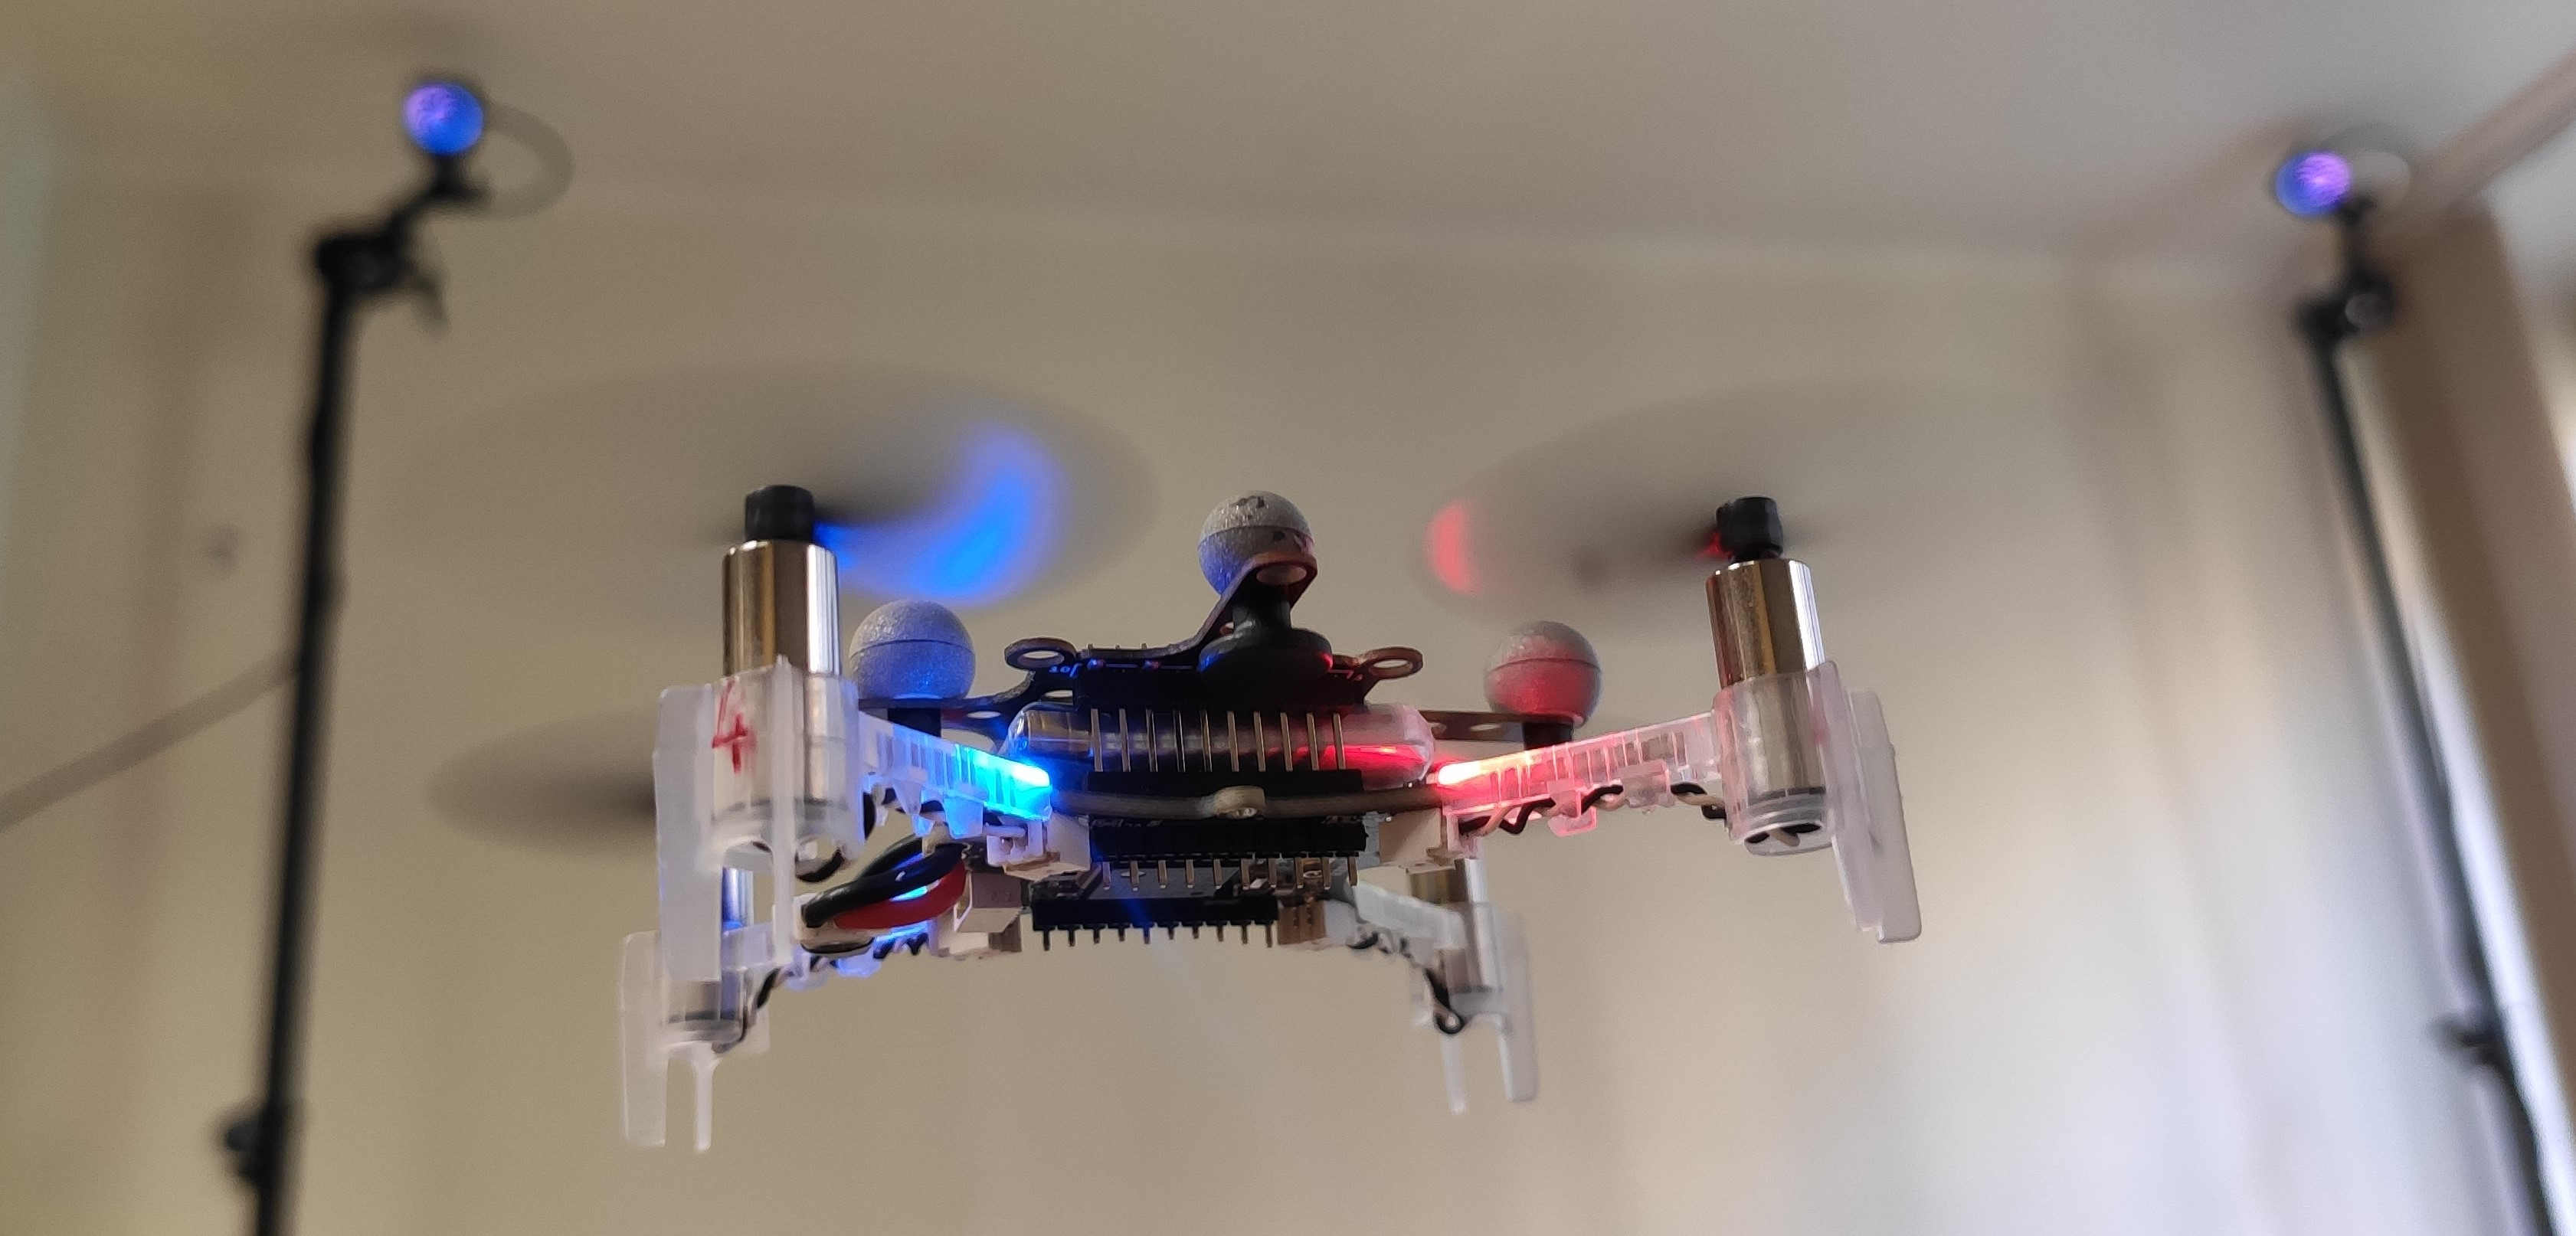
\includegraphics[width=.6\textwidth]{Fig/dronepic.jpg}}
\caption[Experimental setup for the presented measurement results]{Experimental setup for the presented measurement results: 2 OptiTrack Prime 13 infrared cameras and a Crazyflie 2.1 quadcopter with reflective markers.}
\end{figure}

\subsection{Backflip maneuver implementation}\label{sec:implementation}
In the Crazyswarm framework (running on the workstation PC) there are built-in examples for the high-level control of the quadcopter: for example it is enough to call the \verb+takeOff()+, \verb+goTo()+, and \verb+land()+ methods from a script to take off, hover for a specified duration, go to a given point in space, and land -- these commands are sent to the on-board microcontroller through a ROS C++ layer and the Crazyradio PA. In the \verb+.launch+ file of ROS, the user can specify the initial position of the drone, the controller type, state estimator type, logging variables, and other properties. The firmware parameters can be modified mid-flight, for example to adjust controller gains, or switch between controller types.

Our own implementation is a modified version of Crazyswarm, available at the GitHub repository \verb+TDK2021/real_quadcopter/crazyswarm+\footnote{\url{https://github.com/antalpeter1999/TDK2021}}. Our main contributions are in the controller of the firmware (open-loop and geometric control), and in the Python API for high-level commands, and simultaneous control of multiple drones.

\subsubsection{Motor characteristics correction}
In the early implementation phase of the open-loop control, we noticed that there is a significant difference between the characteristics of each motor on a Crazyflie quadcopter. As it is shown in Figure \ref{fig:motors2}, there is more than 3000 rpm and 18\% difference between the angular speed of motor M1 and M2 when the quadcopter is hovering, although the angular speeds should be equal based on the dynamic model. This effect results in the offset of the torque control inputs in all directions, as it is illustrated in Figure \ref{fig:motors} when $t<3$ s.

However, we implemented a correction algorithm to overcome the negative effect on the performance of the backflip. 

\begin{figure}[!h]
  \centering
  \begin{subfigure}[t]{.45\textwidth}
    \centering
    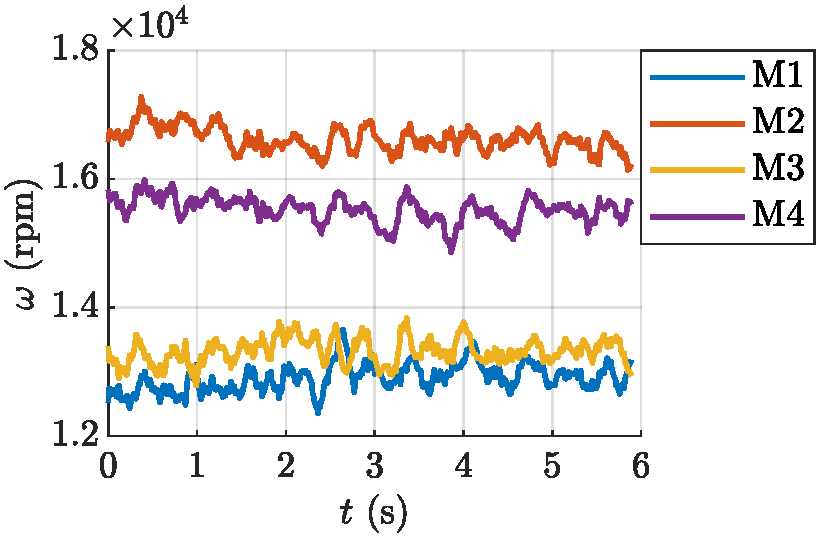
\includegraphics[width=\linewidth]{Fig/motor_offset_2.pdf}
  \caption{Angular speed of the four rotors: in hover mode the values should be equal. }\label{fig:motors2}
  \end{subfigure}
  \hspace{1cm}
  \begin{subfigure}[t]{.45\textwidth}
    \centering
    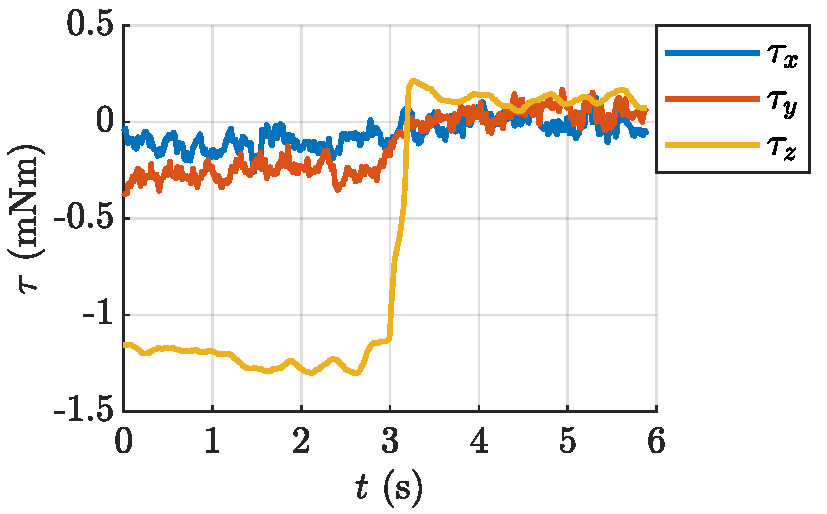
\includegraphics[width=\linewidth]{Fig/motor_offset.pdf}
  \caption{Torque control input: the correction is activated at $t=3$ s, after which the mean of the control inputs are zero.}\label{fig:motors}
  \end{subfigure}%
  \caption{Motor characteristics correction in hovering.}
  \label{fig:motor}
  \end{figure}
%\begin{figure}
%  \centering
%  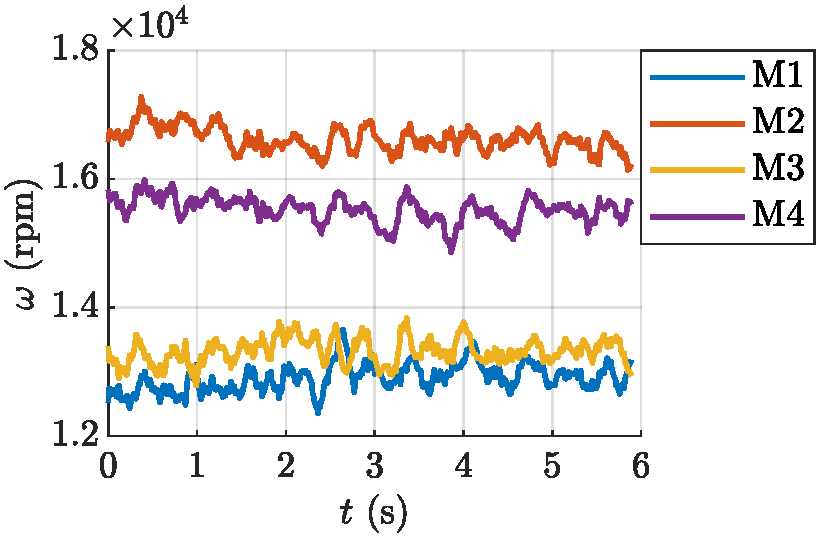
\includegraphics[width=.8\linewidth]{Fig/motor_offset_2.pdf}
%  \caption[Motor offset correction]{Motor characteristics correction in hover mode: the left plot shows the torque control input. The correction is activated at $t=3$ s, after which the mean of the control inputs are zero. The right plot shows the angular speed of each rotor, in hover mode these should be equal. }\label{fig:motors}
%  \end{figure}

\subsubsection{Implementation algorithms}

The high-level script to perform a backflip maneuver is quite simple, because all control algorithms are implemented on-board. However, we need to build and flash the firmware of the quadcopter MCU after every change in the source code, therefore parameter setting and execution of high-level tasks is easier using Python scripts. The steps of the high-level script to perform the backflip are illustrated in Algorithm \ref{alg:hl}.

\begin{algorithm}
  \caption{High-level script executed on the ground control PC}
  \label{alg:hl}
  \begin{algorithmic}[1]
    \State Send parameters to the Crazyflie: controller type (open-loop or geometric), trajectory information, controller gains
    \State Take off and hover at the initial point of the flip
    \State Start the flip maneuver, and wait until it is over
    \State Land
  \end{algorithmic}
  \end{algorithm}

The evaluation of the open-loop control law, i.e. the calculation of control inputs from the current time has small computational cost, therefore it is practical to be implemented on-board. The implementation is detailed in Algorithm \ref{alg:open}, the maneuver is triggered from the ground station with a high-level command, it is executed automatically, and the quadcopter ends in hovering mode afterwards.
%In our implementation of this controller, the user only needs to set the value of \verb+isFlipControl+ variable to true, the quadcopter immediately starts the flip maneuver, and then automatically switches back to PID control. The parameters of the maneuver are sent to the drone before taking off (at the beginning of the high-level script). %The flip control policy is implemented within the innermost loop of the PID control code, therefore it runs at 500 Hz.
\begin{algorithm}
  \caption{Open-loop control on-board implementation}
  \label{alg:open}
  \begin{algorithmic}[1]
    \State Hover with PID control, wait for ground station command to start the backflip
    \State Lift with PID control to gain momentum
      \While {the flip is not over}
      \State Decide in which section we are (out of the 5 in Fig. \ref{fig:sections})
      \State Apply the control input of the current section based on \eqref{eq:openinp}
    \EndWhile
    \State Stabilize the quadcopter with PID control
    \State Get back to initial position
  \end{algorithmic}
  \end{algorithm}

The second control approach, i.e. reference trajectory tracking with geometric control is also implemented on-board. The coefficients of the designed trajectory represented by 7th degree polynomials, and the corresponding time span are saved to a csv file after the simulations. In the Python API, it is loaded and sent to the Crazyflie with the tuned controller gains, before taking off. The on-board implementation of the control approach is detailed in Algorithm~\ref{alg:geom}. Similarly to the open-loop approach, the command to start the maneuver comes from the ground station, and then the backflip is performed automatically.
\begin{algorithm}
  \caption{Geometric tracking control on-board implementation}
  \label{alg:geom}
  \begin{algorithmic}[1]
    \State Hover with geometric control, wait for ground station command to start the backflip
    \State Lift with geometric control to gain momentum
      \While {the flip is not over}
      \State Get the current state from the state estimator module
      \State Get the setpoint by evaluating the reference trajectory
      \State Calculate the control inputs from the control law \eqref{eq:geomlaw}
      \State Apply the control inputs to the motors
    \EndWhile
    \State Stabilize the quadcopter with geometric control
    \State Get back to initial position
  \end{algorithmic}
  \end{algorithm}


 %When the user wants to start the backflip maneuver, similarly to the open-loop method, only needs to set the value of \verb+isFlipControl+ to true. The on-board algorithm then starts executing the previously saved trajectory, switches to pitch reference from yaw reference, and switches back after the maneuver is over. 

%A big advantage of the on-board control is that the maneuver can be performed by multiple quadcopters simultaneously without any problems coming from communication delays and lost packages between the ground control PC and the drone microcontroller.

\subsection{Experimental results}

Experiments to perform the backflip maneuver started with the open-loop method. Firstly, we used the optimal parameter set from \eqref{eq:optparam}, but due to the differences of the simulation model and the real quadcopter dynamics, the drone almost performed a double flip with these parameters, and the stabilization was not successful at the end of the maneuver. After realizing the differences between the measurements and the simulations, we manually tuned the parameters so that the flip is executed with minimal final state error. The refined experimental parameter set is
\begin{align*}
    P^\mathrm{exp} = \begin{bmatrix}
U_1^\mathrm{exp} & t_1^\mathrm{exp} & t_3^\mathrm{exp} & U_5^\mathrm{exp}& t_5^\mathrm{exp}
\end{bmatrix} ^\top =  \begin{bmatrix}
14.29 & 0.2 & 0 & 14.29 & 0.075
\end{bmatrix}^\top.
\end{align*}
The measurement results are displayed in Figure \ref{fig:openmeas}, showing the trajectory of the position and orientation during the maneuver. It is important to note that an additional lift phase is added to the implementation to gain enough vertical velocity and height, because the quadcopter falls a significant distance in the recovery phase. During the additional lift phase the PID controller is used to achieve exact vertical lifting and horizontal orientation.

Figure \ref{fig:openmeas} shows that the flip is executed with almost zero final error in the pitch, and also quite small position error. Compared to the simulation displayed in Figure~\ref{fig:opensimu}, the maximal displacement from the origin in $x$ direction is around a half, and in $z$ direction around double. The difference is due to the manual refinement of the motion sequence parameters, and the uncertainties of the simulation model. It is important to note that the performance of the open-loop controller is very sensitive to uncertainties in the dynamics and initial conditions. For example, if the flip maneuver begins when the orientation of the quadcopter is not exactly horizontal, the stability can be lost at the recovery phase. Hence the open-loop flip is only successful in about 6-7 trials out of 10.
\newpage
\begin{figure}
\centering
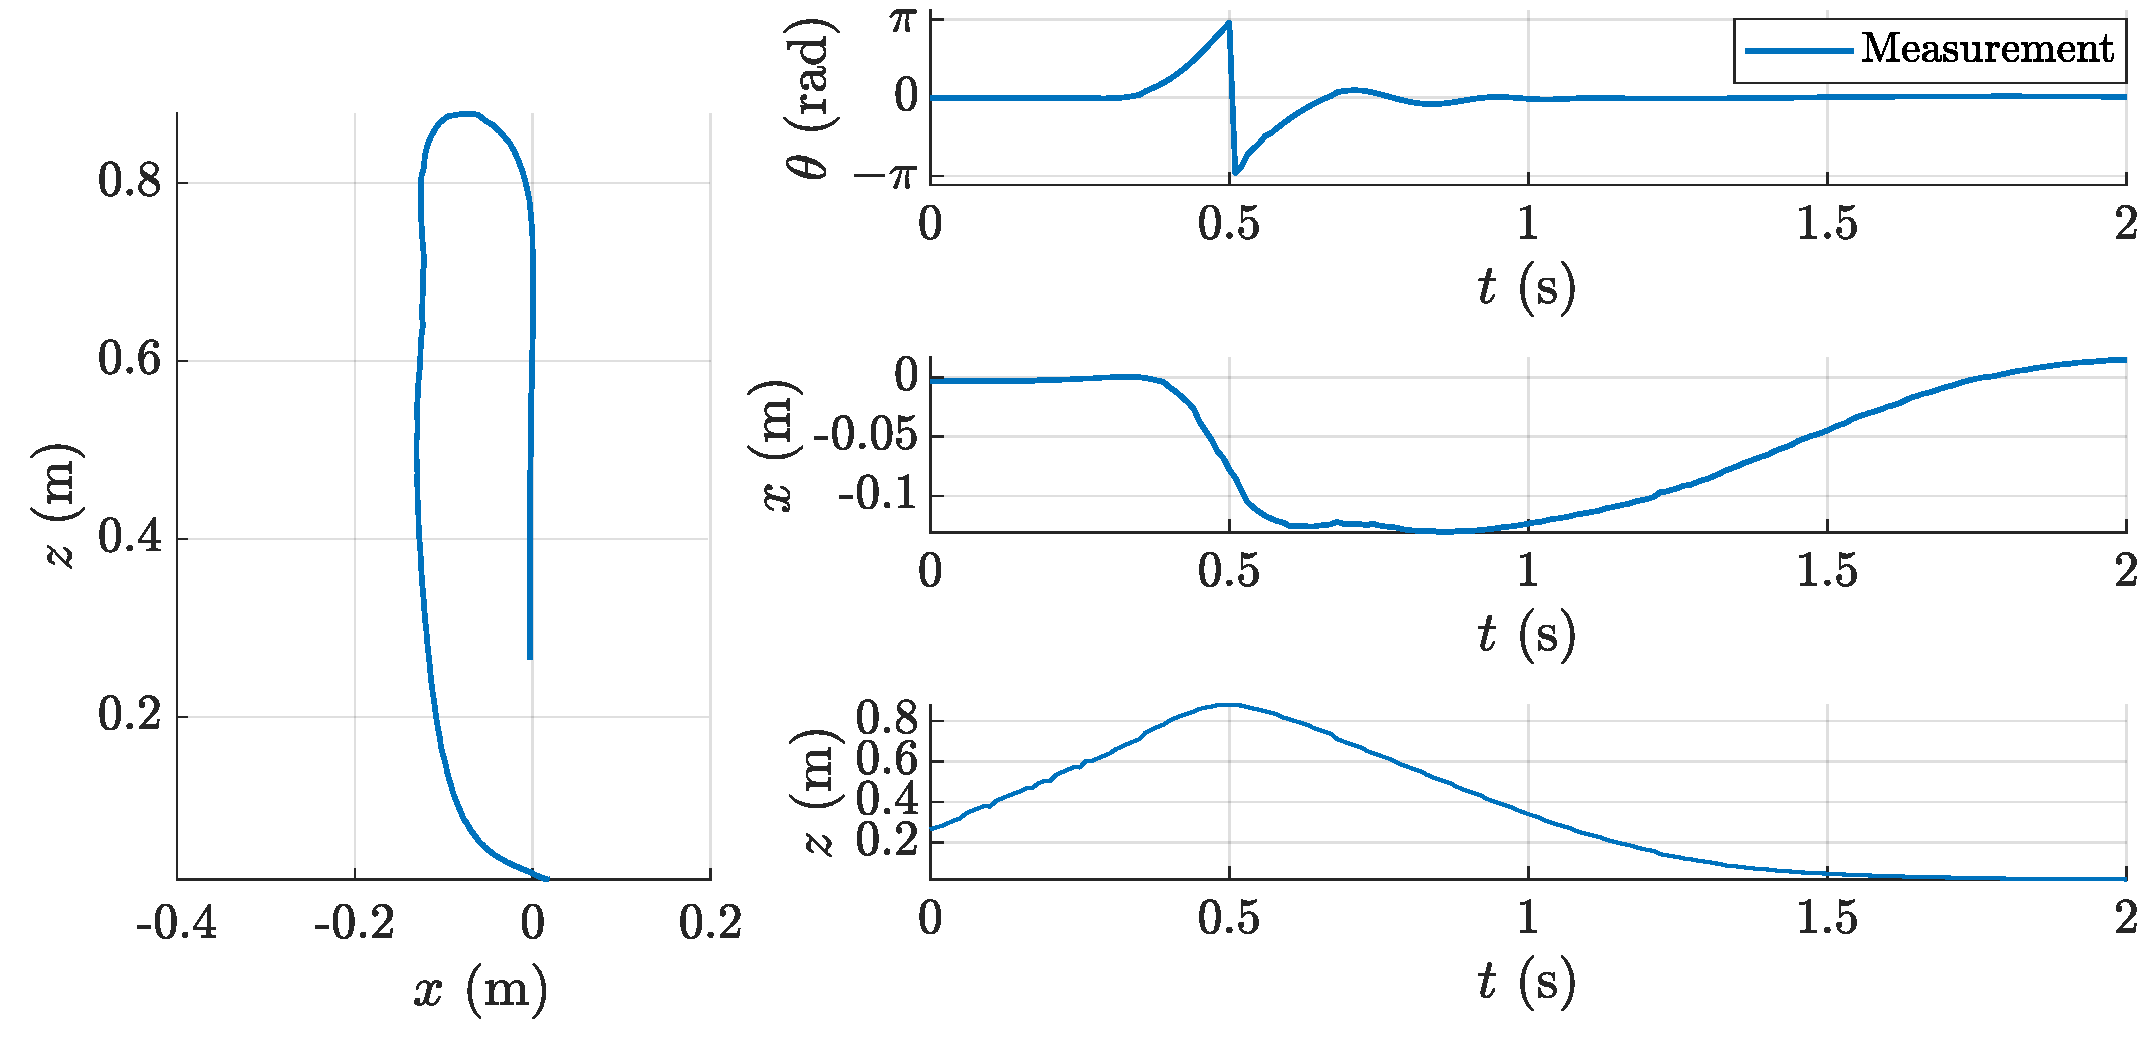
\includegraphics[width=.8\linewidth]{Fig/openmeast.pdf}
\caption[Backflipping measurement results with open-loop control]{Backflipping measurement results with open-loop control. The position and pitch angle of the quadcopter are displayed.}\label{fig:openmeas}
\end{figure}

\begin{figure}
\centering
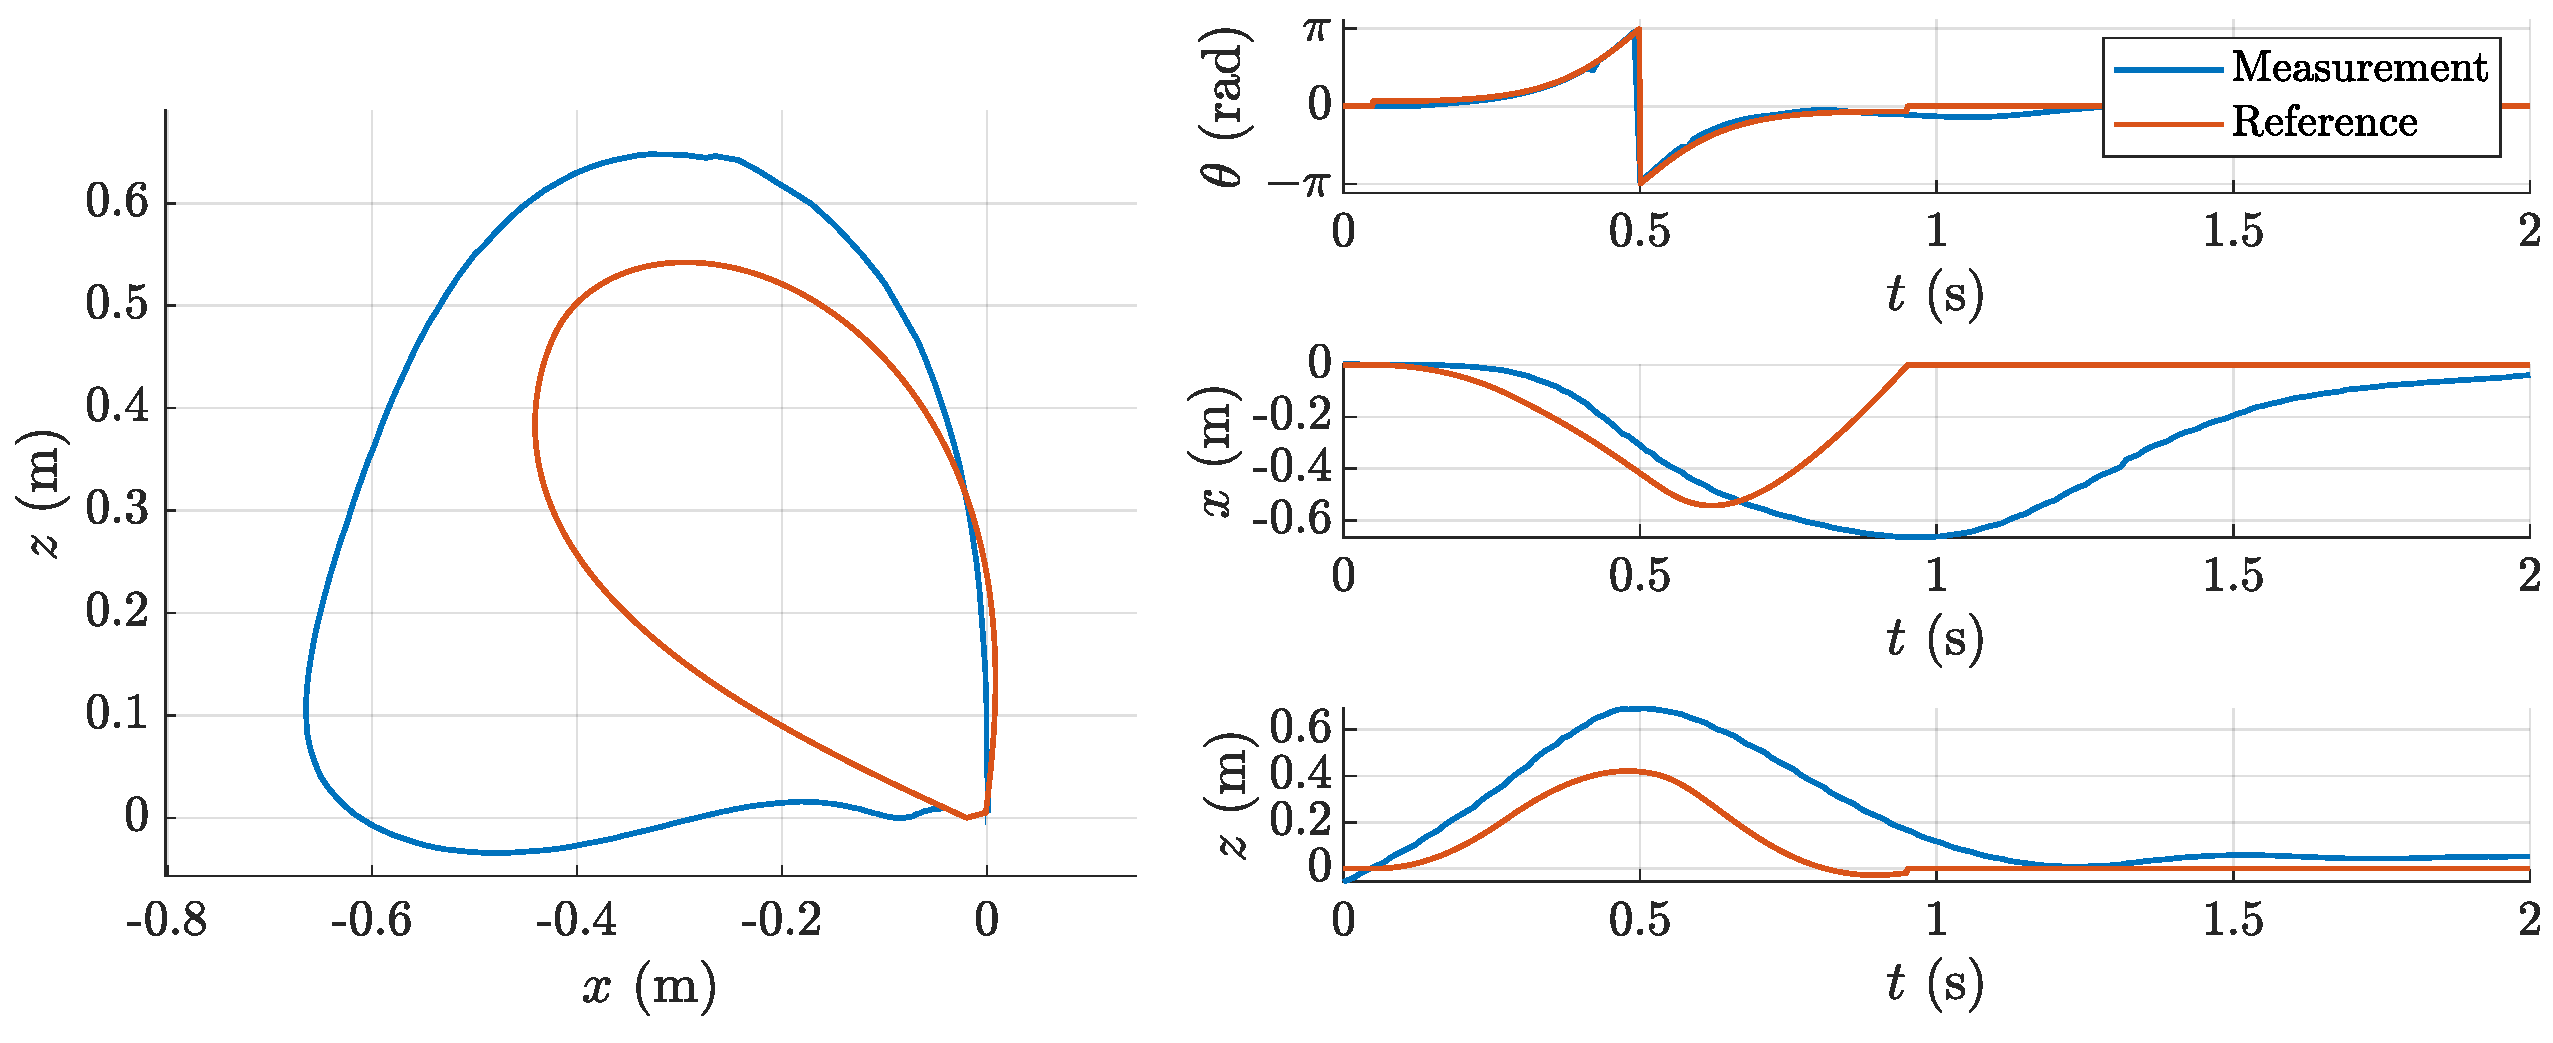
\includegraphics[width=.8\linewidth]{Fig/geommeast2.pdf}
\caption[Backflipping measurement results with geometric control]{Backflipping measurement results with geometric control. The trajectories show that the maneuver is performed successfully, and the drone gets back to the initial position at the end.}\label{fig:geommeas}
\end{figure}

The experimental results of the backflipping with geometric control are displayed in Figure~\ref{fig:geommeas}. The most important part of reference tracking is the pitch angle $\theta$, because a fast, stable and accurate attitude tracking is required to perform the flip maneuver, and recover successfully. As it is shown on the upright plot of the measurement results, the pitch is very close to the reference. 

However, the error of the position tracking is significantly higher during the maneuver, both in $x$ and $z$ directions. There are many possible reasons of the high positioning error, the following are the most likely. Firstly, we assume at the trajectory design that the orientation is equal to the reference at all time steps, which is not far from reality, but there is always a non-zero attitude tracking error. It was another assumption of trajectory design that the derivative of the control input can be arbitrarily large. However, when the quadcopter is upside down, a near-minimal collective thrust is required, and shortly after a near-maximal thrust to recover and follow the reference, as it is illustrated in Figure \ref{fig:geommeas}. Small DC motors are usually modelled as first order systems with a small time constant, but here the transient can be significant, the motor needs time to build up the thrust of the propellers. The third possible explanation is also connected to model uncertainty. The modelling of aerodynamic effects such as blade flapping, induced drag or downwash \cite{quad_model} are very complex, therefore we exclude these terms from the dynamic model, however, they can have a negative effect on the performance of the feedback controller when performing the backflip maneuver.

In spite of the imperfect position tracking, the geometric controller is able to perform the backflip maneuver exactly the same way ten out of ten times, which indicates that it is significantly more robust than the open-loop method. Even with smaller changes on the dynamic behaviour of the quadcopter (e.g. replacing a reflective marker with a larger one), the maneuver is performed successfully and the drone remains stable.



\begin{figure}
\setlength{\fboxsep}{0pt}%
\setlength{\fboxrule}{1pt}
\centering
\begin{subfigure}{.45\textwidth}
  \centering
  \fbox{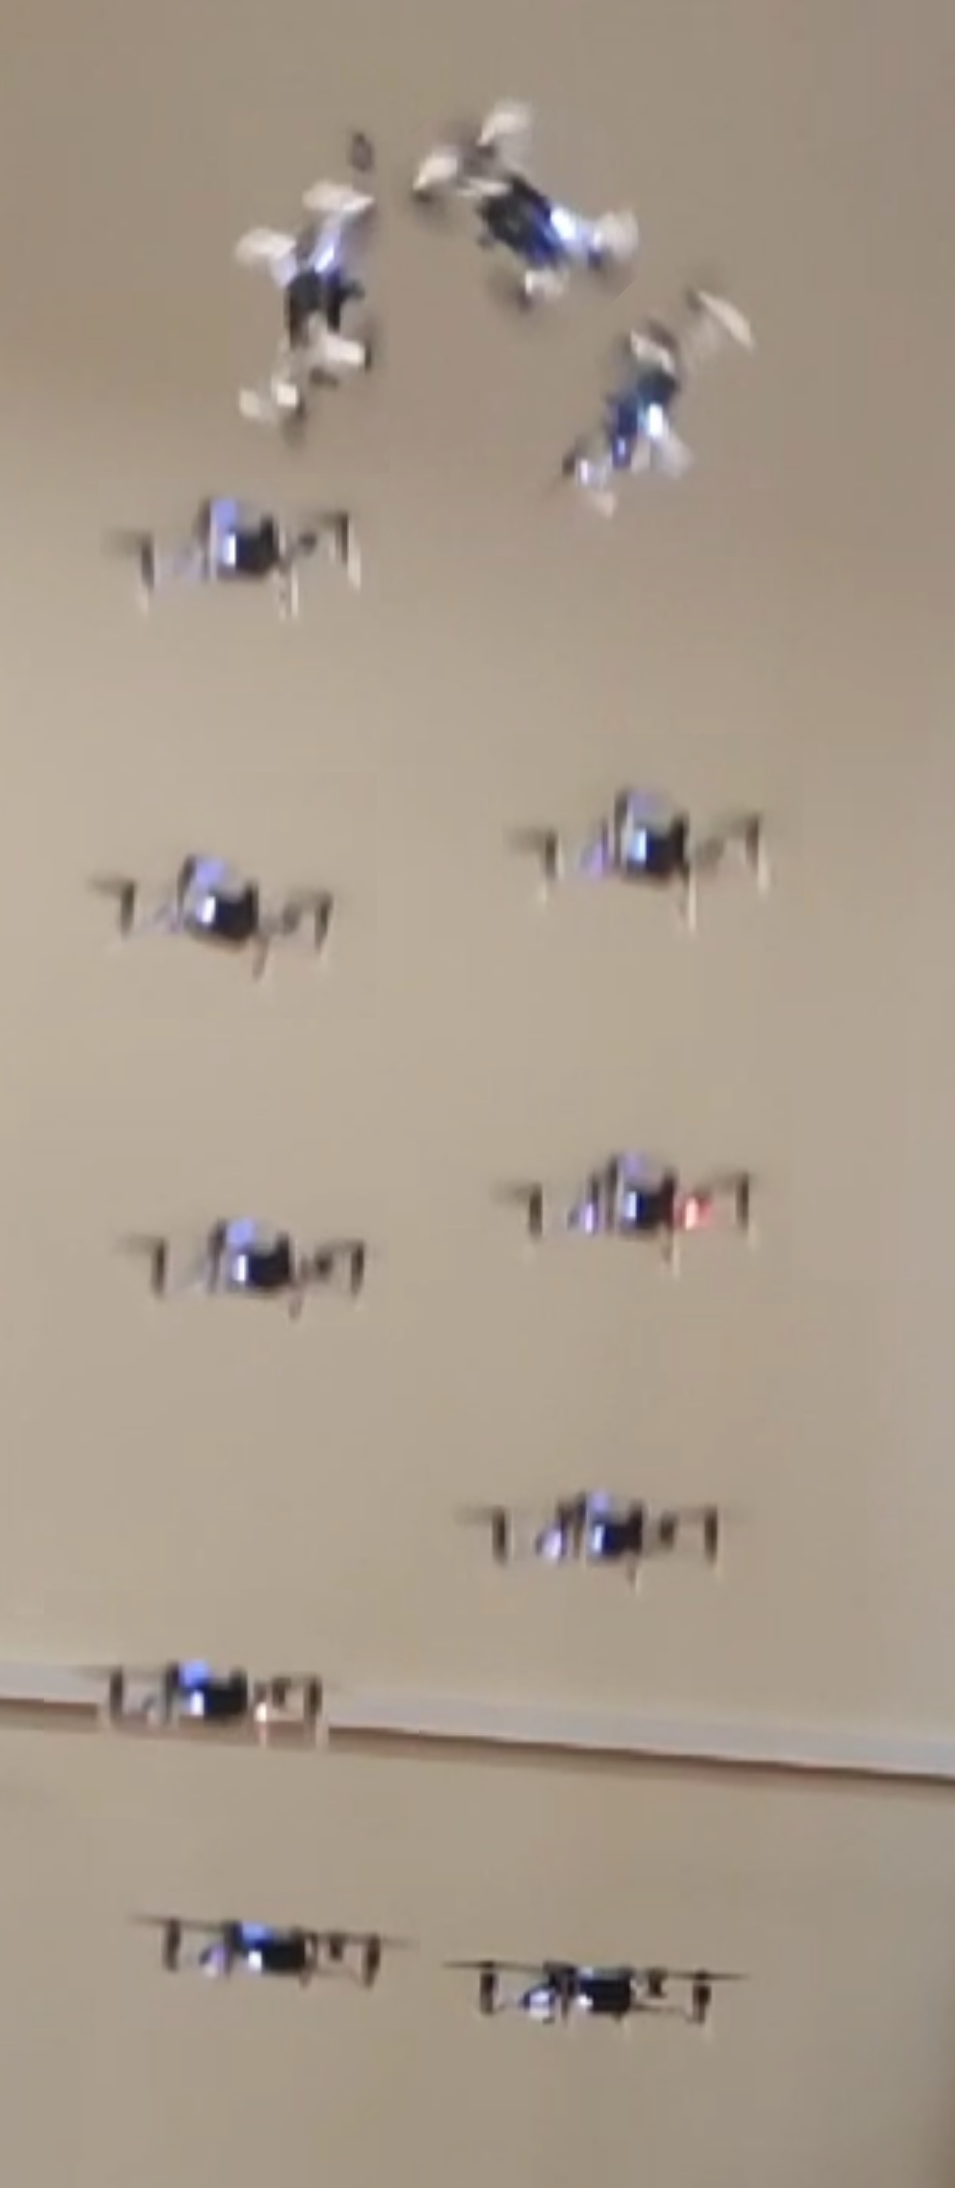
\includegraphics[height=6cm]{Fig/opencomp.png}}
  \caption{Optimization-based open-loop control, the trajectory is displayed in Fig. \ref{fig:openmeas}.}
  \label{fig:sub1}
\end{subfigure}%
\hspace{1cm}
\begin{subfigure}{.45\textwidth}
  \centering
  \fbox{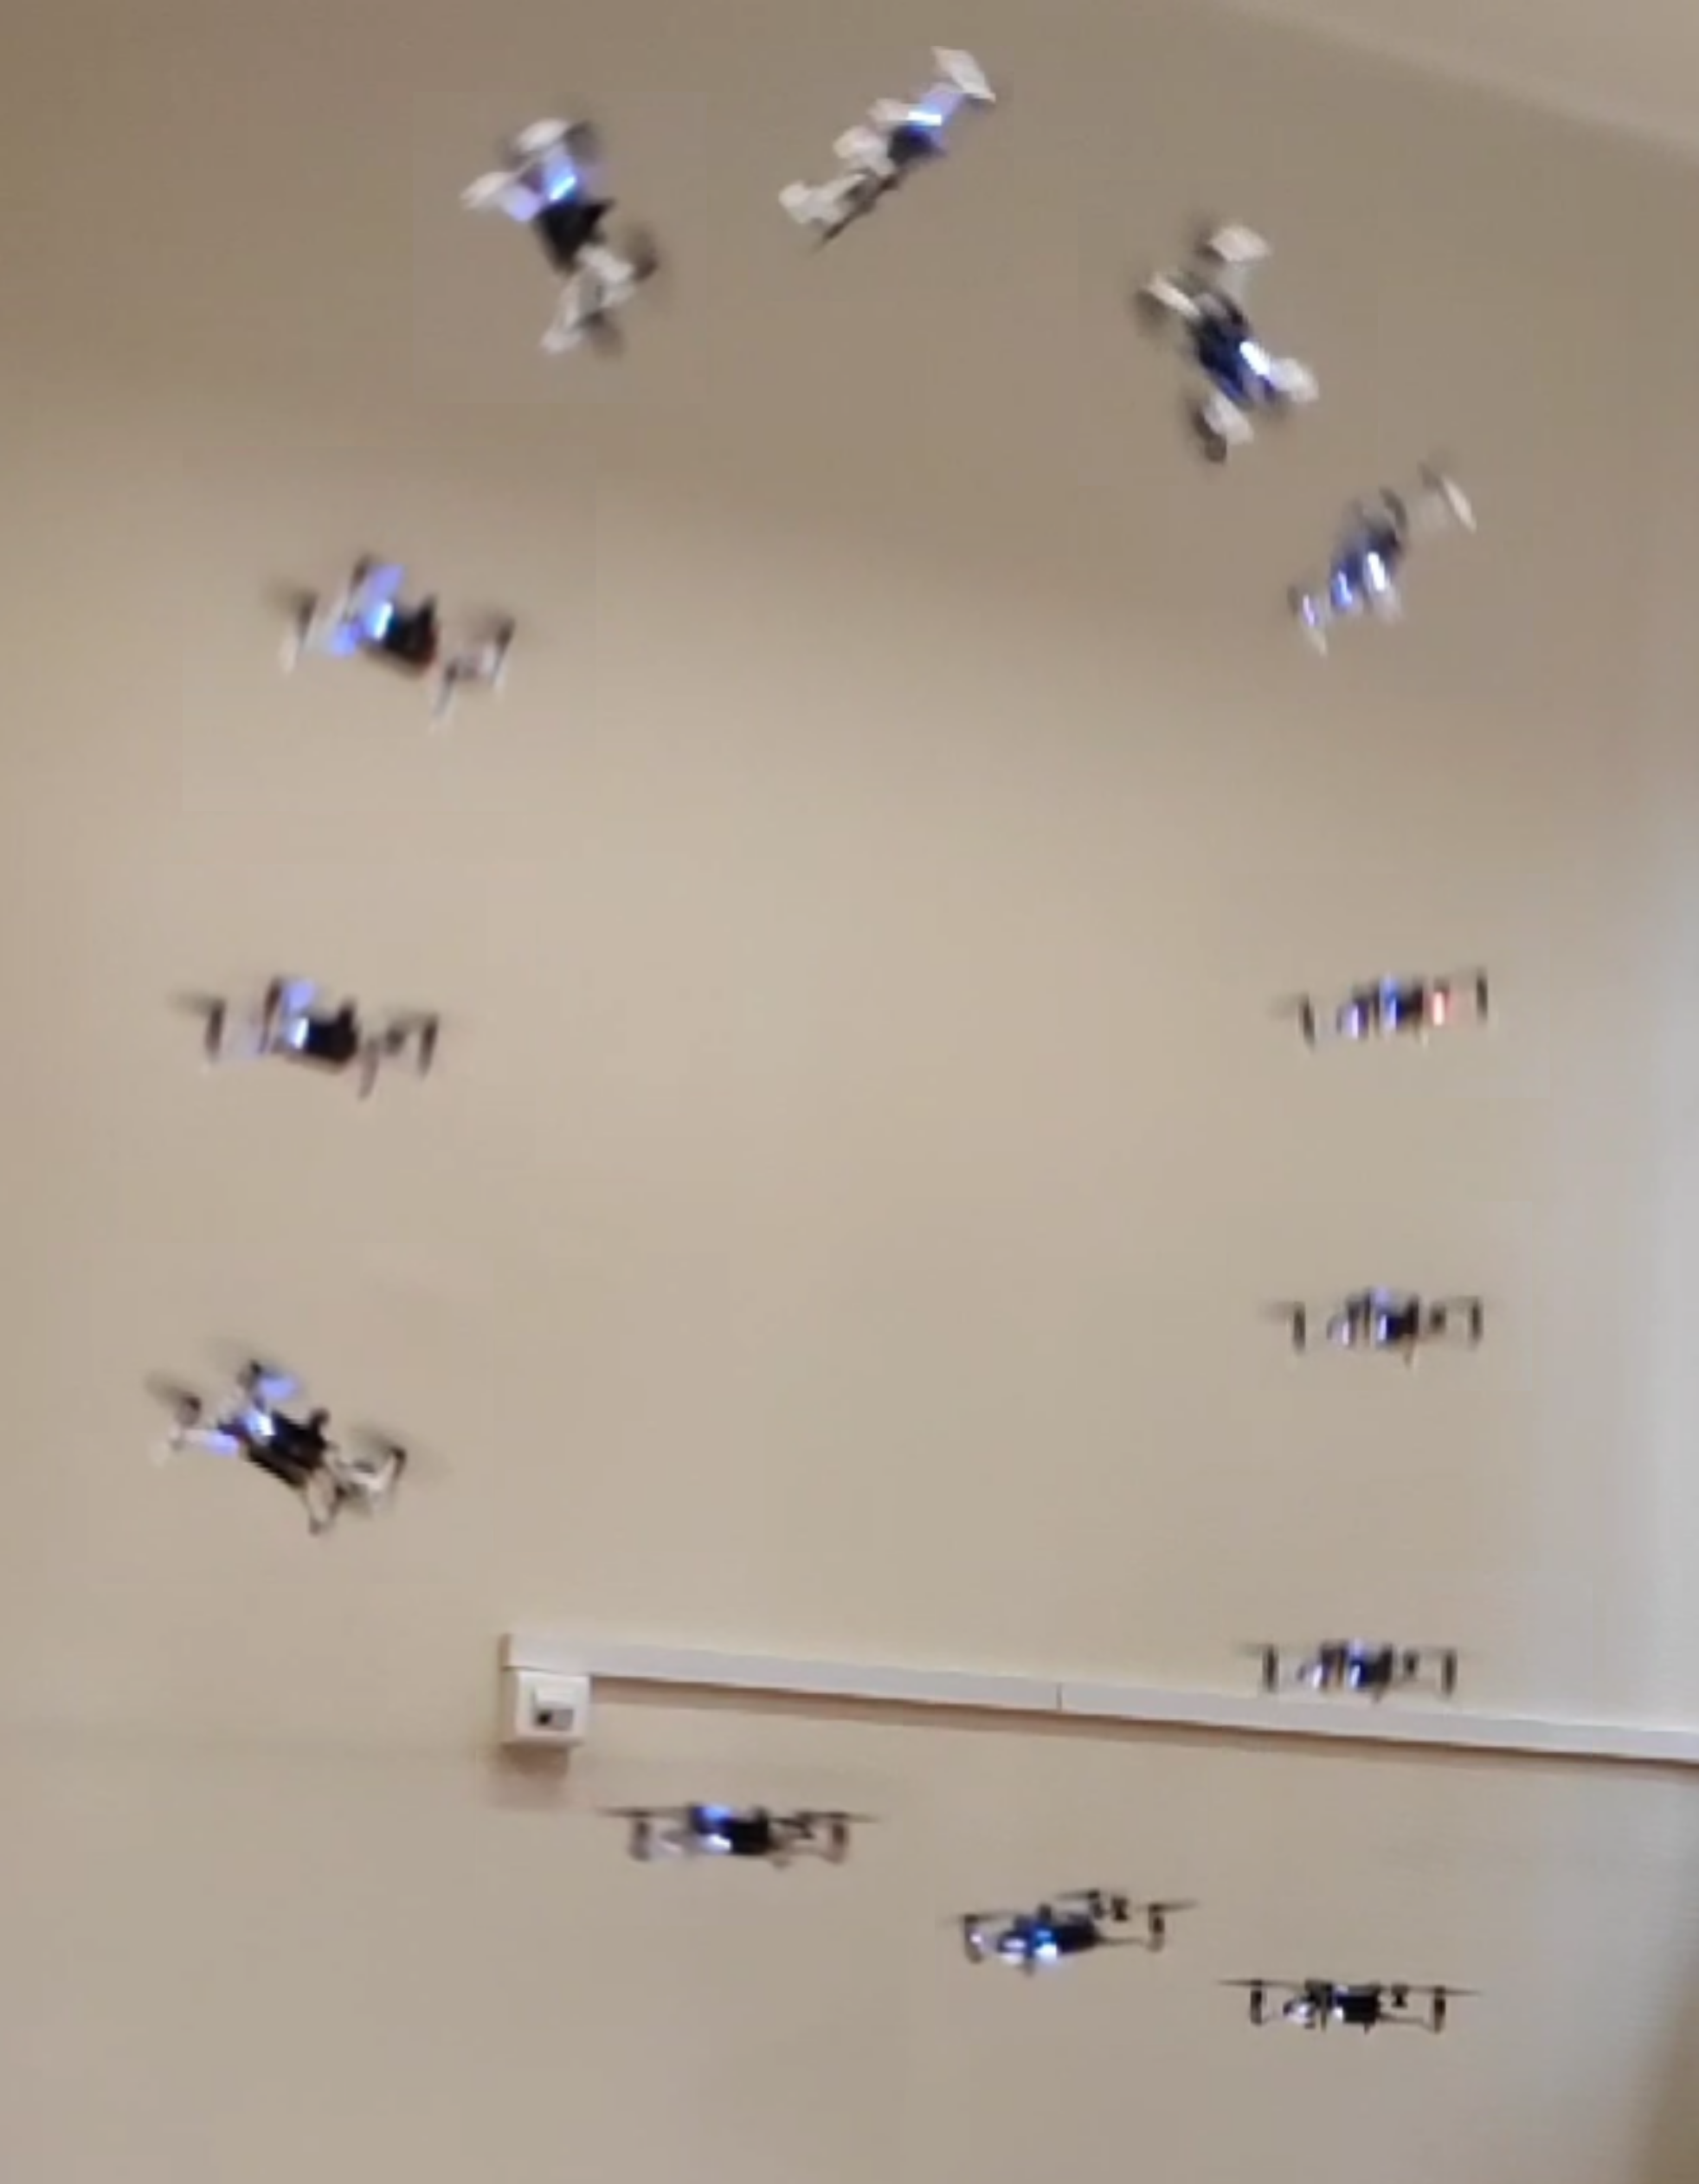
\includegraphics[height=6cm]{Fig/geomcomp.png}}
  \caption{Geometric reference tracking control, the trajectory is displayed in Fig. \ref{fig:geommeas}.}
  \label{fig:sub2}
\end{subfigure}
\caption[Composite images of the measurement results]{Composite images of the measurement results with both proposed control methods. A video of the measurements is available at \url{https://youtu.be/AhqfXZ-CPqM}.}
\label{fig:test}
\end{figure}

\subsection{Robustness and scalability for multiple drones}
The presented measurement results are satisfactory for both control methods, the quadcopter performed a backflip maneuver successfully. However, the open-loop approach is very sensitive to parameter uncertainties, therefore it needs specific tuning for each Crazyflie. Moreover, it is also sensitive to initial conditions, because the open-loop control input is the same even if there is a nonzero angle or displacement at the starting point. Hence the quality of the maneuver often varies even with the manually refined parameters. Due to the inconsistency of the performance, we could not apply the open-loop control for simultaneous flip with multiple drones.

However, geometric tracking control overcomes the problematics caused by parameter uncertainties using feedback, providing a highly robust and consistent performance for the backflip maneuver. Utilizing the robustness of the control approach, the maneuver has been implemented for simultaneous backflipping with three drones. A video of the acrobatic maneuver is available at \url{https://youtu.be/AhqfXZ-CPqM}. The implementation of the simultaneous flip differs from the single maneuver discussed in Section \ref{sec:implementation} only in the high-level script. The trajectory of each drone during the maneuver is evaluated relatively to their initial position and orientation, making it easy to extend the single flip implementation. % In the high-level script we send each drone to their initial pose, and send the command to start the flip. Afterwards, the quadcopters hover at the initial pose and wait for the next command, for example to land.

The scalability of the proposed control algorithms for other types of quadcopters (e.g. medium or large-sized) is out of the scope of this work, however, the possibilities are briefly discussed in the followings. The open-loop method is applied in \cite{LSICRA2010} to a medium-sized drone successfully, therefore we are convinced that our modified version could also be applied to other types. Geometric control is even more general than the open-loop approach, it is applied not only for different types of quadcopters \cite{turpinkumar2011}, but also for other autonomous systems, such as robotic manipulators \cite{bullo2004}. Hence the proposed control algorithms could be used in industrial applications, as well.